\providecommand{\myrootdir}{..}
\documentclass[\myrootdir/main.tex]{subfiles}

\begin{document}

\chapter{Empirical Comparison}
\label{sec:study}
To investigate when PBE, CTS and KWS are suited to retrieve chunks from CI build logs we evaluate them on the \emph{LogChunks} data set.
This chapter describes our study design and which metrics we measure to answer our research questions.
In the presentation of the results, we first focus on each of the three techniques and later compare them against each other.


\begin{figure}[htbp]
	\centering
	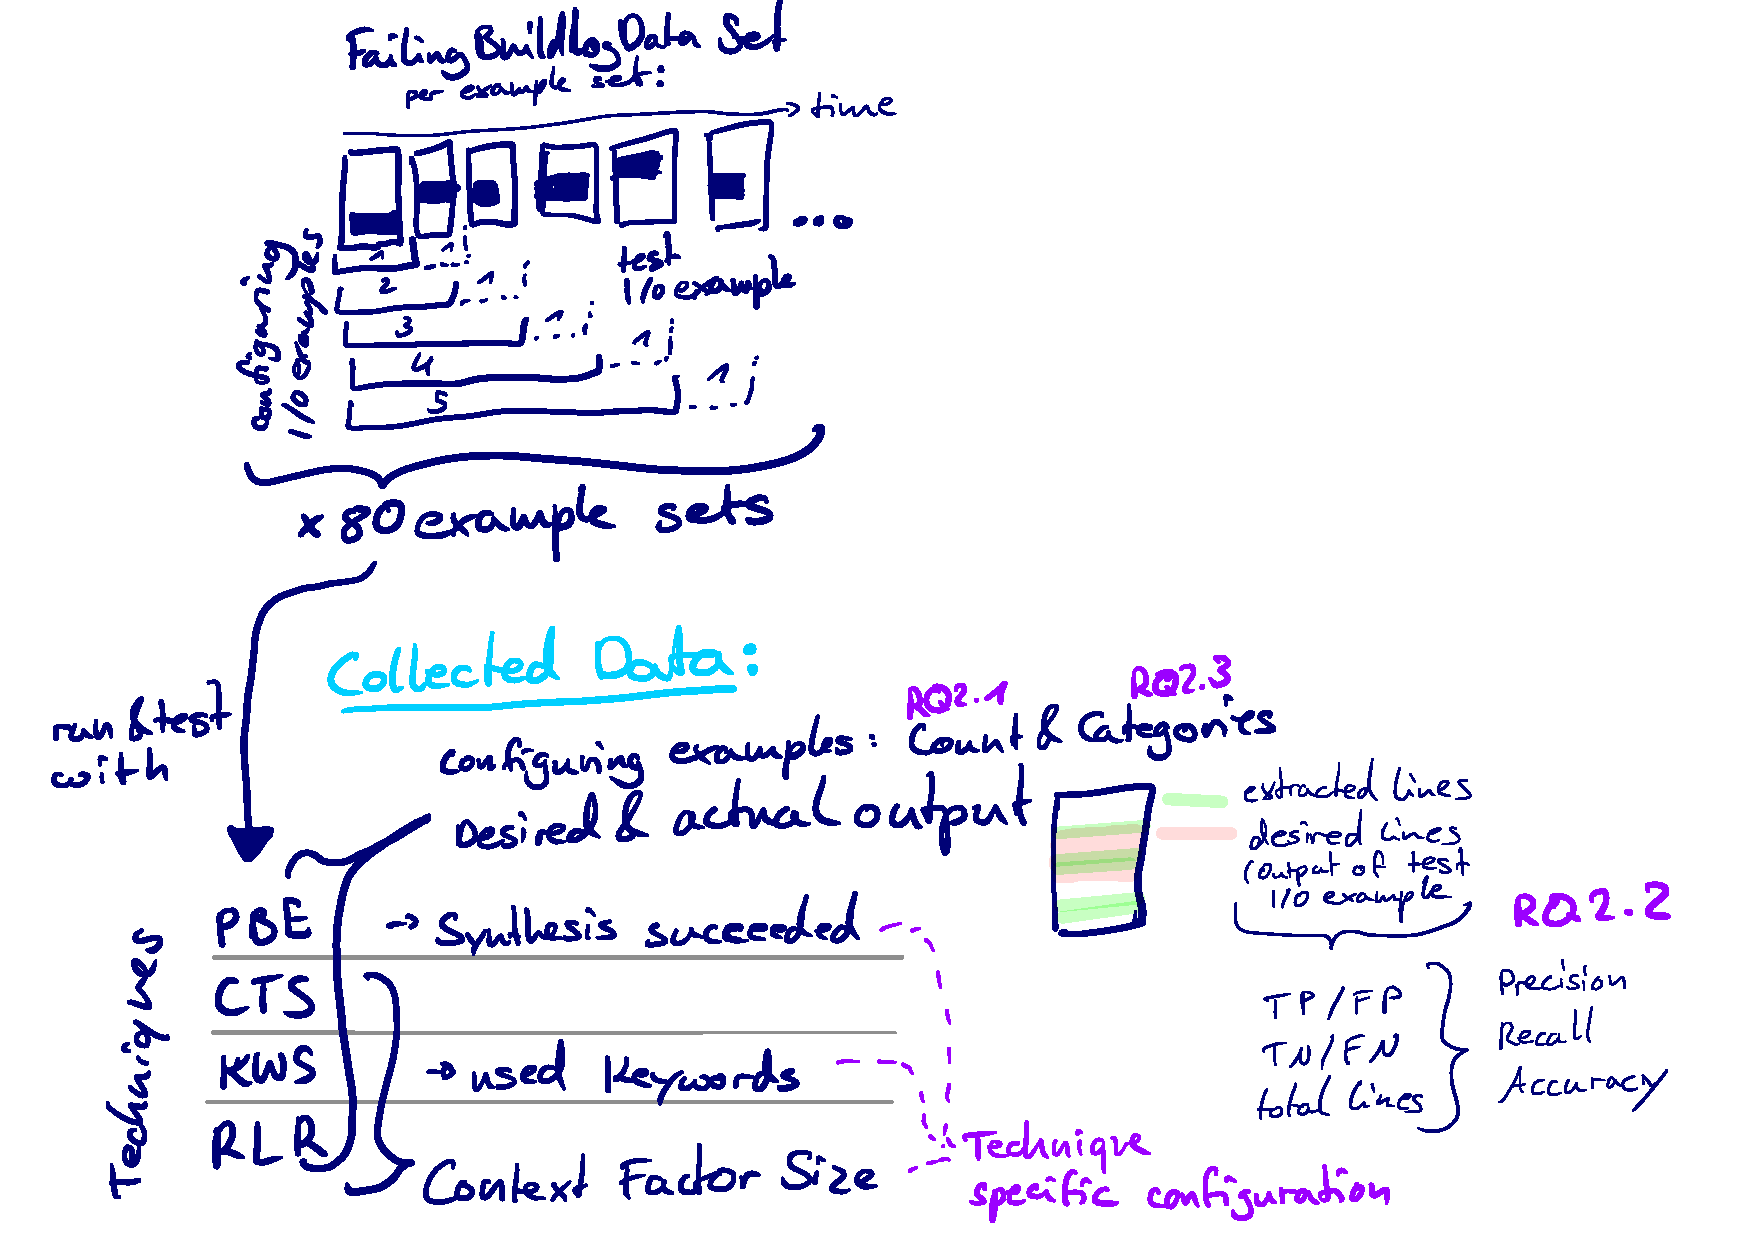
\includegraphics[width=\textwidth, clip]{img/study-design.pdf}
	\caption{Study design of our technique comparison study}
	\label{fig:study}
\end{figure}


\begin{simplebox}{Research Questions}
\begin{itemize}
  \item[\textbf{RQ1:}] Which criteria influence the suitability of a chunk retrieval technique for CI build logs?
  \item[\textbf{RQ2:}] Under which conditions are PBE, CTS, and KWS suited to retrieve information from CI build logs?
  \item[\textbf{RQ2.1:}] How many examples do PBE, CTS, and KWS need to perform best?
  \item[\textbf{RQ2.2:}] How structurally similar do the examples for PBE, CTS and KWS need to be for the techniques to be applicable?
  \item[\textbf{RQ2.3:}] How accurate are the retrievals of PBE, CTS, and KWS?
\end{itemize}
\end{simplebox}

\section{Study Design}
For the comparison, we evaluate the three chunk retrieval techniques PBE, CTS and KWS, described in Sections~\ref{sec:expl-pbe},\ref{sec:expl-ts} and~\ref{sec:expl-skws}.
RLR, explained in Section~\ref{sec:expl-rlr}, acts as a baseline for the comparison.
We run four techniques on the Examples from \emph{LogChunks}.
\paragraph{Training and Test Set}
We use \emph{LogChunks} as the data set for our study.
For each one of 80 repositories it contains about 10 build logs, manually labeled with the substring describing the reason the build failed.
In addition to that, it contains keywords to search for that substring and which structural category the substring belongs to.

For each repository in \emph{LogChunks}, we split the examples chronologically into training and test set.
Therefore, we train on examples from past build logs and test on future build logs.
\paragraph{RQ 2.1: Size of Training and Test Set}
To analyze how many examples the chunk retrieval techniques need to perform best, we evaluate the techniques with different training set sizes.
We train each technique with one to five examples from each of the repositories within \emph{LogChunks}.
The size of the test set is one.
\paragraph{RQ 2.2: Recording Structural Categories}
To determine how structurally similar the examples for the chunk retrieval techniques need to be, we record the structural categories of the examples in the training and test sets.
\paragraph{RQ2.3: Accuracy Metrics}
To measure the accuracy of the retrieved chunks we save the output lines of the chunk retrieval run on the input of the test example ($retrievedlines$).
As oracle in our evaluation, we save the desired lines from the output of the test example ($desiredlines$).

We calculate the following metrics:
\begin{itemize}
	\item True positives: $TP = desiredlines \cap retrievedlines$
	\item Precision: $Precision =  \frac{\# TP}{\# retrievedlines}$
	\item Recall: $Recall = \frac{\# TP}{\# desiredlines}$
	\item Successful retrieval: $true\ if\ Recall = 1$
\end{itemize}

Precision of a chunk retrieval describes which proportion of the retrieved lines were not targeted.
Recall of a chunk retrieval describes which proportion of the targeted lines were retrieved.
Throughout the presentation and discussion of our results we keep these two metrics separate, as they might have a different weight when choosing a suitable technique for a task.
We define a successful retrieval as one where all desired lines were extracted, therefore when recall is one.

Recall and precision of CTS and KWS vary with the number of lines selected for retrieval.
We evaluate the effect of varying the number of extracted lines by multiplying the average number of lines present in the training examples with a \emph{retrieval size factor} from 0.5 to 2.5 in steps of 0.5.

\section{Results}
This section presents the results for PBE, CTS and KWS separately.
Afterwards we compare the three techniques with each other and RLR as baseline.

\subsection{Program Synthesis by Example (PBE)}
Figure~\ref{fig:failure-reason-PBE} shows the results of the PBE runs in our evaluation.
Out of the 400 runs, 5 per each one of the 80 example sets, PBE extracted all the desired lines in 138 cases.
Figure~\ref{fig:failure-reason-PBE} shows that in 89 further cases a program was also successfully synthesized, though in 59 cases the synthesized program yielded no output at all.
In 30 cases the synthesized program did not extract all of the desired lines and had an average recall of 28\%.
In 173 cases the PROSE program synthesis could not synthesize a regular expression program that is consistent with all of the training examples.

Figure~\ref{fig:failure-reason-categorycount-PBE} shows the results of PBE runs compared to the number of structural categories present in the training examples.
It shows that the program synthesis is more likely to succeed when there are few categories present in the training examples.
When two structural categories are present, PROSE could in most cases not synthesize a program consistent with all training examples.
For three or more present categories PROSE could never synthesize a consistent program.

Figure~\ref{fig:recall-precision-examplecount-sythesisworked-PBE} shows precision and recall of runs where PBE could synthesize a program consistent with all training examples.
When the training set size increases from one to two, recall increases by 24\% and precision increases by 10\%.
For two or more training examples the recall stays around 75\% and precision around 96\%.

\begin{figure}[htbp]
		\centering
		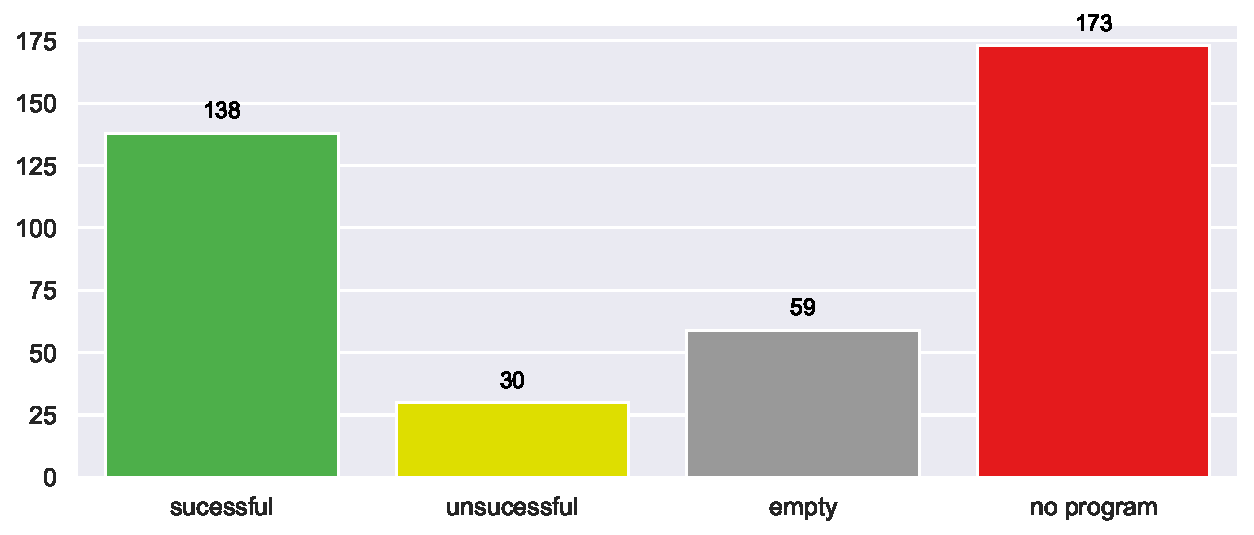
\includegraphics[width=0.5\textwidth, clip]{img/big-study/failure-reason-PBE.pdf}
		\caption{Results of chunk retrieval with PBE}
		\label{fig:failure-reason-PBE}
\end{figure}

\begin{figure}[htbp]
		\centering
		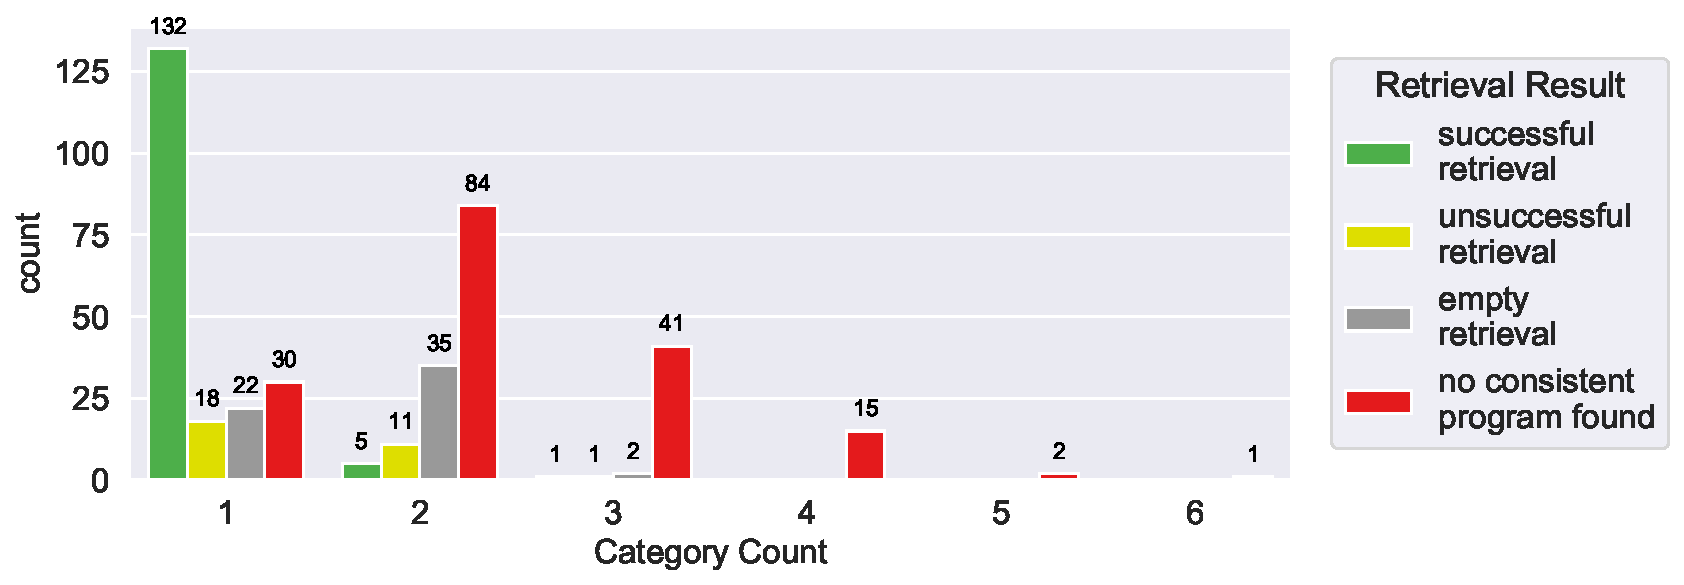
\includegraphics[width=0.75\textwidth, clip]{img/big-study/failure-reason-categorycount-PBE.pdf}
		\caption{Results of chunk retrieval with PBE for increasing number of structural categories in the training and test set}
		\label{fig:failure-reason-categorycount-PBE}
\end{figure}

\begin{figure}[htbp]
		\centering
		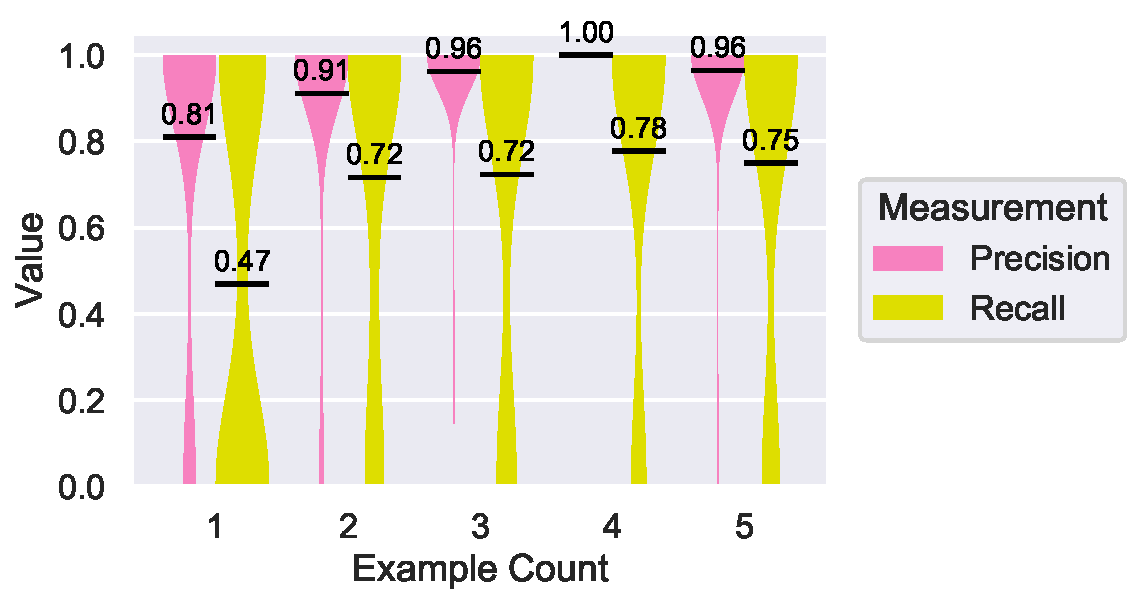
\includegraphics[width=0.75\textwidth, clip]{img/big-study/recall-precision-examplecount-sythesisworked-PBE.pdf}
		\caption{Precision and recall of chunk retrieval when PBE could synthesize a consistent program compared with the size of the training set}
		\label{fig:recall-precision-examplecount-sythesisworked-PBE}
\end{figure}

\begin{figure}[htbp]
		\centering
		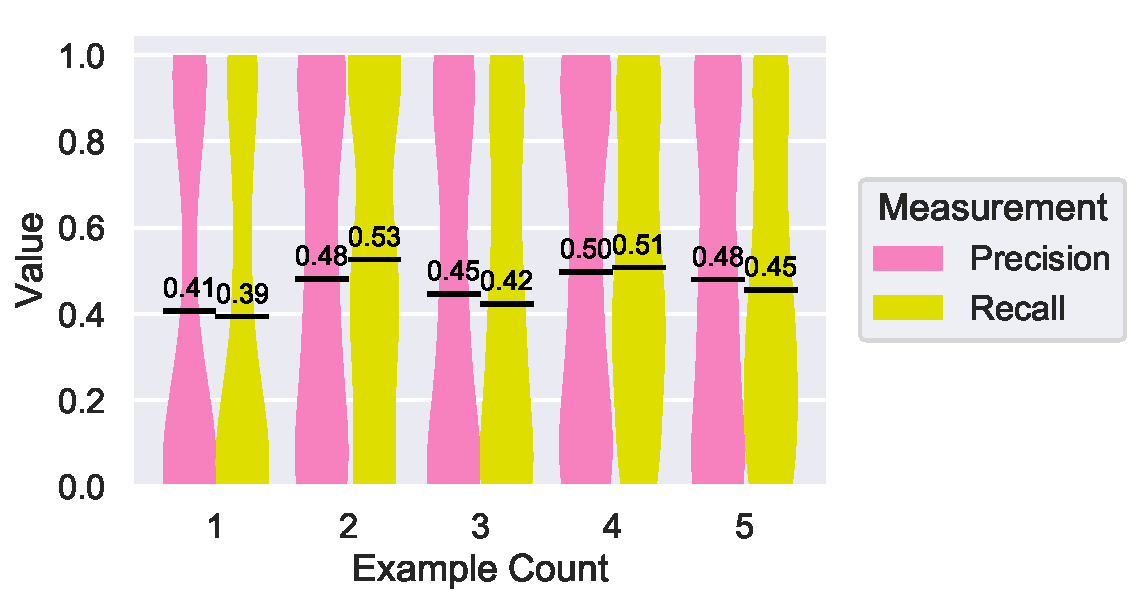
\includegraphics[width=0.75\textwidth, clip]{img/big-study/recall-precision-examplecount-CTS.pdf}
		\caption{Precision and recall of chunk retrieval with CTS for increasing training set size}
		\label{fig:recall-precision-examplecount-CTS}
\end{figure}

\begin{figure}[htbp]
		\centering
		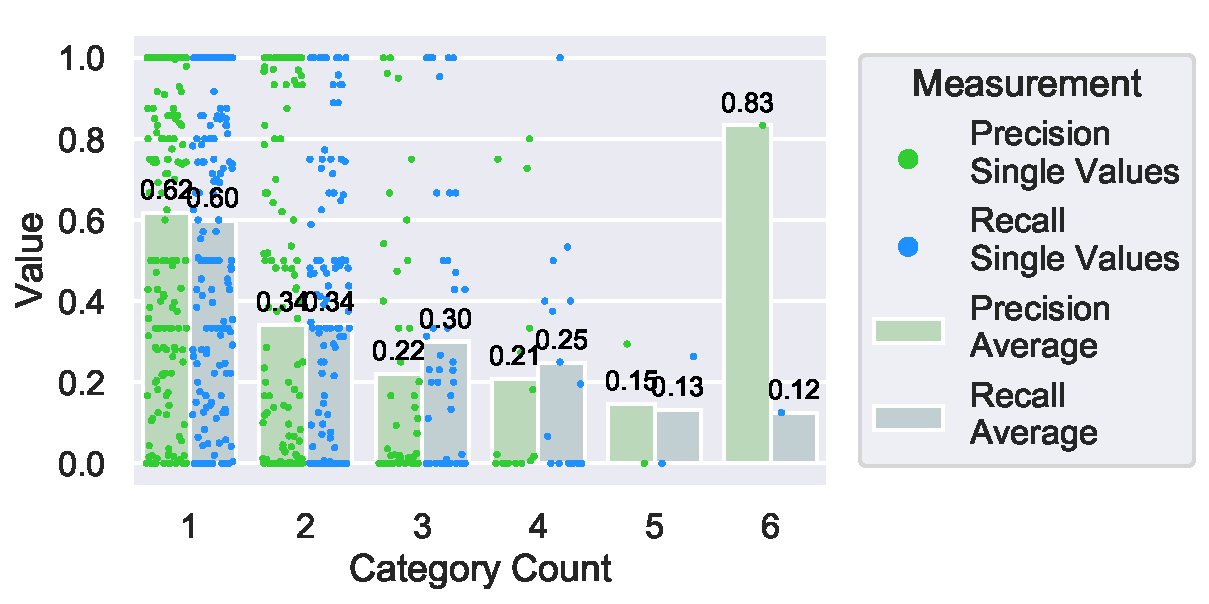
\includegraphics[width=0.75\textwidth, clip]{img/big-study/recall-precision-categorycount-CTS.pdf}
		\caption{Precision and recall of chunk retrieval with CTS for increasing number of structural categories in the training and test set}
		\label{fig:recall-precision-categorycount-CTS}
\end{figure}

\begin{figure}[htbp]
		\centering
		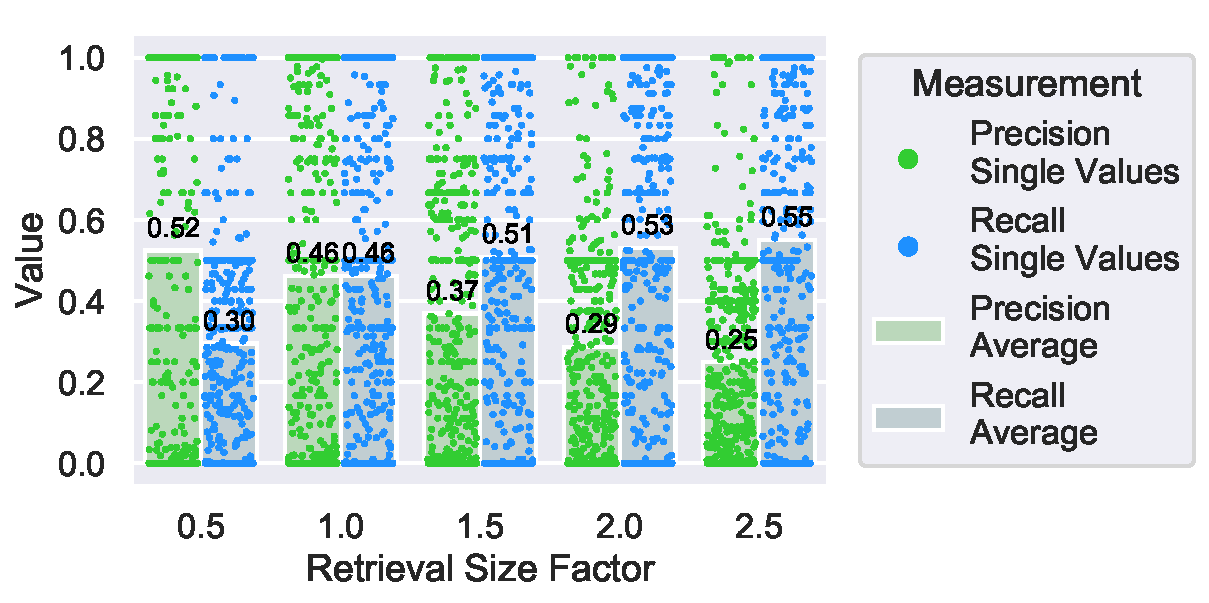
\includegraphics[width=0.75\textwidth, clip]{img/big-study/contextsizefactor-precision-recall-CTS.pdf}
		\caption{Precision and recall of chunk retrieval with CTS compared to retrieval size factors}
		\label{fig:contextsizefactor-precision-recall-CTS}
\end{figure}

\subsection{Common Text Similarity (CTS)}
Figure~\ref{fig:recall-precision-examplecount-CTS} presents precision and recall of chunk retrieval using CTS for an increasing number of training examples.
When using one to five training examples, the size of the training set has no noticeable influence on recall and precision of the chunk retrieval with CTS.

Figure~\ref{fig:recall-precision-categorycount-CTS} shows the same measurements for an increasing number of structural categories in the training and test examples.
With increasing category count, precision and recall decrease.
Especially for more than four categories present we have no chunk retrieval runs where all desired lines were extracted.

Figure~\ref{fig:contextsizefactor-precision-recall-CTS} shows the effect of the retrieval size factor on precision and recall of chunk retrieval runs with CTS\@.
The precision ranges from 52\% when retrieving half expected number of lines to 25\% when 2.5 times the expected number of lines.
The recall ranges from 30\% to 55\%.

\begin{figure}[htbp]
		\centering
		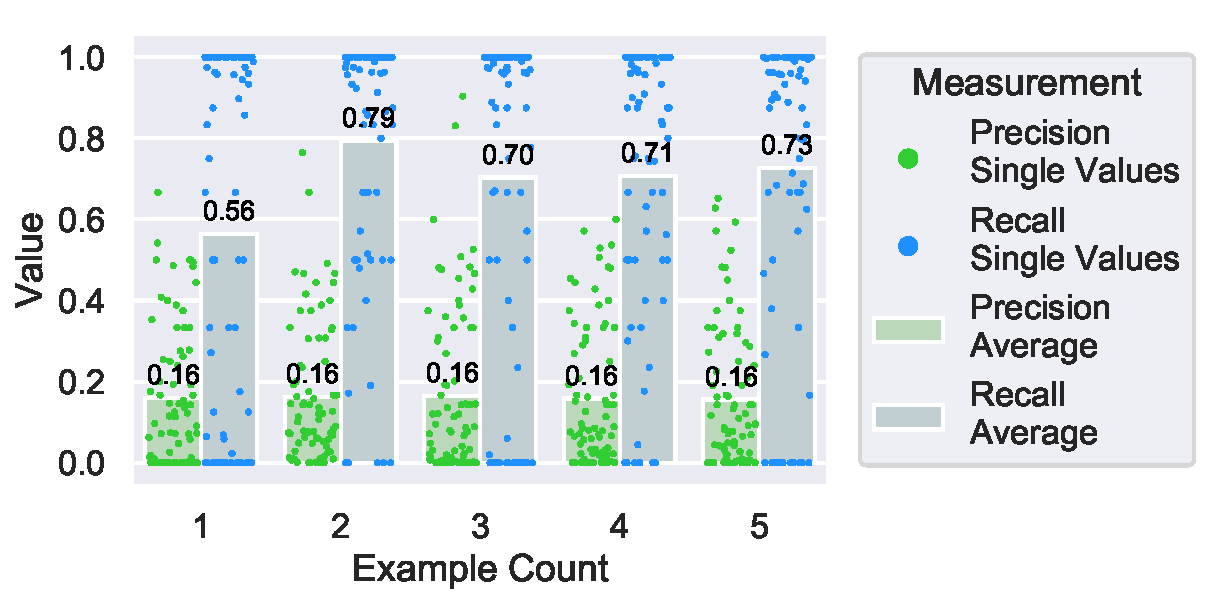
\includegraphics[width=0.75\textwidth, clip]{img/big-study/recall-precision-examplecount-KWS.pdf}
		\caption{Precision and recall of chunk retrieval with KWS for increasing training set size}
		\label{fig:recall-precision-examplecount-KWS}
\end{figure}

\begin{figure}[htbp]
		\centering
		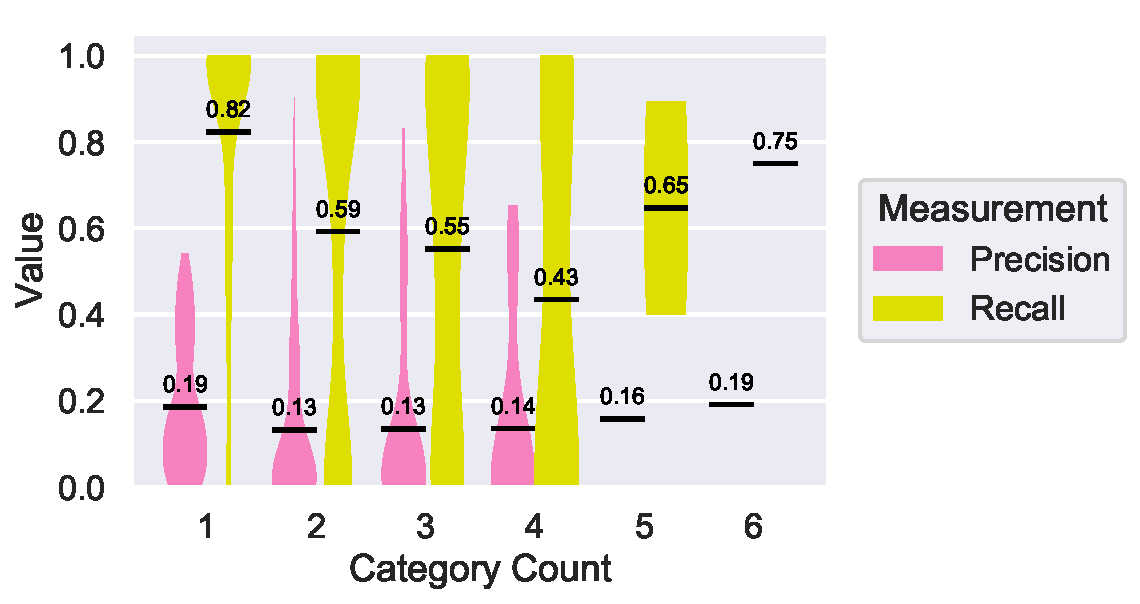
\includegraphics[width=0.75\textwidth, clip]{img/big-study/recall-precision-categorycount-KWS.pdf}
		\caption{Precision and recall of chunk retrieval with KWS for increasing number of structural categories in the training and test set}
		\label{fig:recall-precision-categorycount-KWS}
\end{figure}

\begin{figure}[htbp]
		\centering
		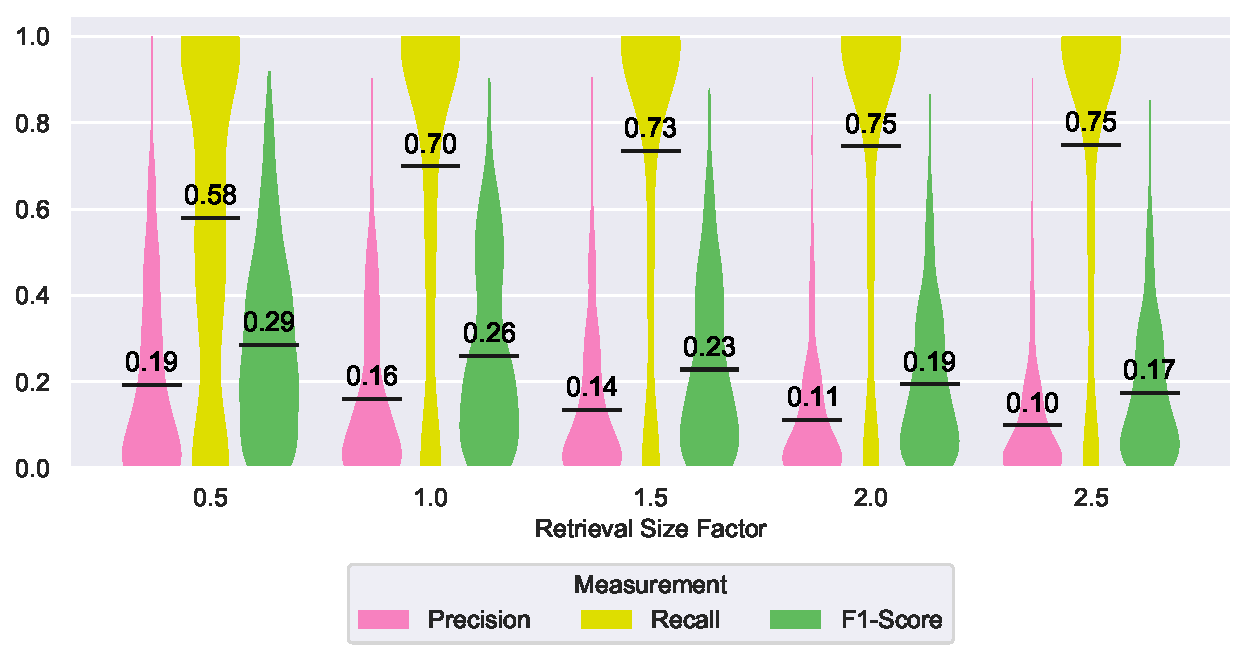
\includegraphics[width=0.75\textwidth, clip]{img/big-study/contextsizefactor-precision-recall-KWS.pdf}
		\caption{Precision and recall of chunk retrieval with KWS compared to retrieval size factor}
		\label{fig:contextsizefactor-precision-recall-KWS}
\end{figure}

\subsection{Keyword Search (KWS)}
Figure~\ref{fig:recall-precision-examplecount-KWS} presents precision and recall of chunk retrieval using KWS for different numbers of training examples.
The recall increases by about 12\% when increasing the size of the training set to more than one example, while the precision stays constant at around 16\%.

Figure~\ref{fig:recall-precision-categorycount-KWS} shows the same measurements for increasing number of structural categories in the training and test examples.
For more than one structural category in the training and test examples the recall decreases about 20\% and the precision decreases about 6\%.
For more than two structural categories no clear trend visible in precision and recall for an increasing amount of categories in the training and test examples.

Figure~\ref{fig:contextsizefactor-precision-recall-KWS} shows the effect of the retrieval size factor on precision and recall of chunk retrieval runs with KWS\@.
The precision is 19\% when retrieving half expected number of lines. On average 9\% of the lines in the build log are retrieved then.
When 2.5 times the expected number of lines, the precision decreases to 10\% and a quater of the lines in the build log are retrieved on average.
The recall ranges from 58\% to 75\%.

\begin{figure}[htbp]
		\centering
		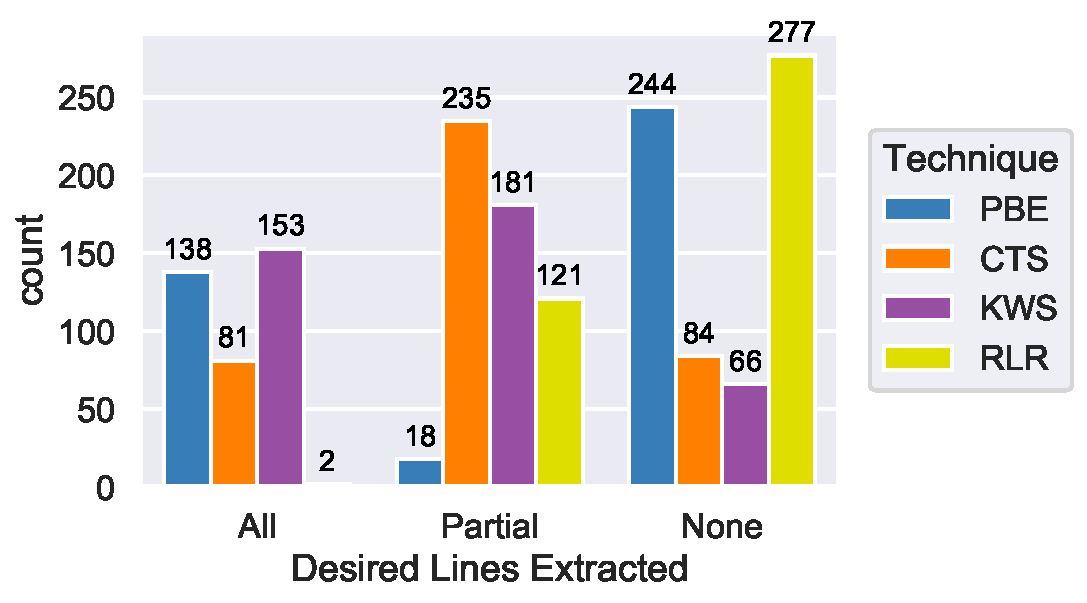
\includegraphics[width=0.75\textwidth, clip]{img/big-study/success-partial-all.pdf}
		\caption{Success of chunk retrievals for all techniques}
		\label{fig:success-partial-all}
\end{figure}

\begin{figure}[htbp]
		\centering
		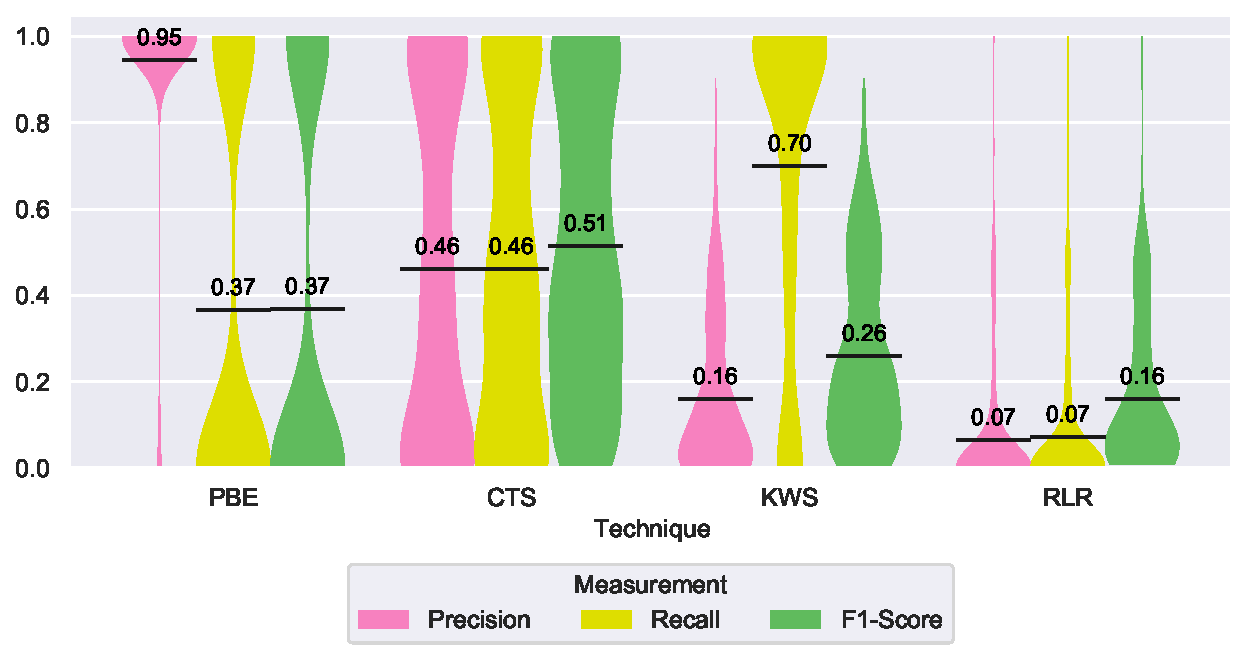
\includegraphics[width=0.75\textwidth, clip]{img/big-study/recall-precision-all.pdf}
		\caption{Precision and recall of all techniques compared}
		\label{fig:recall-precision-all}
\end{figure}

\begin{figure}[htbp]
	\centering
		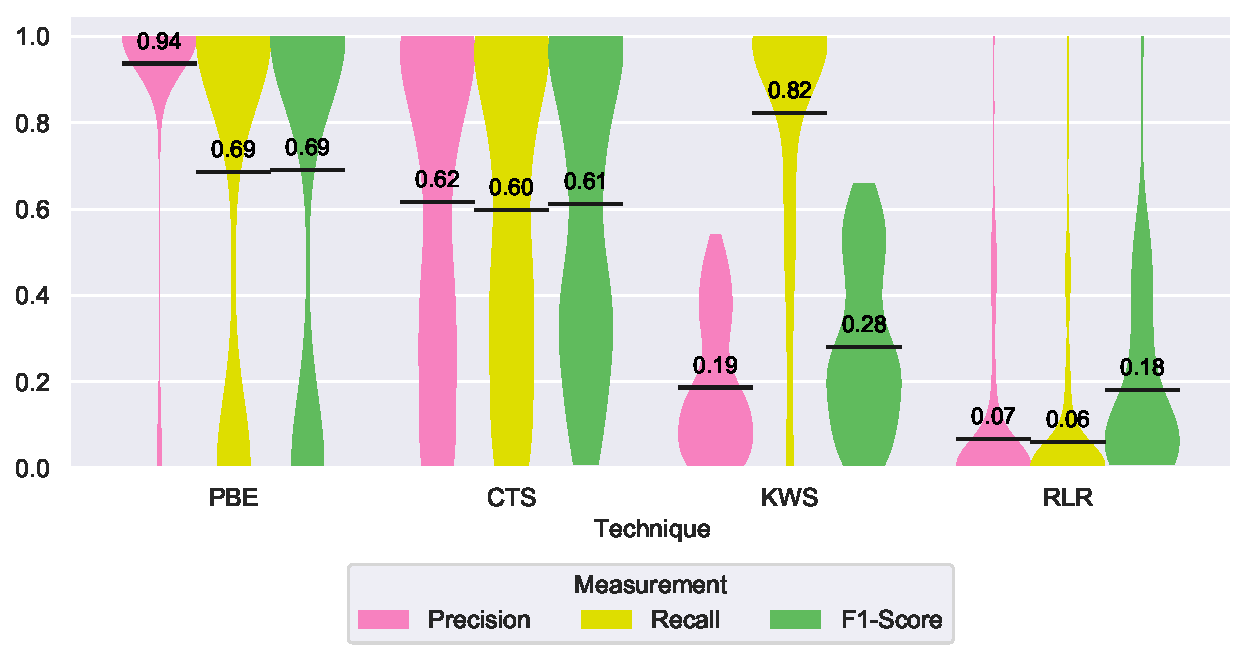
\includegraphics[width=0.75\textwidth, clip]{img/big-study/recall-precision-singlecategory-all.pdf}
		\caption{Precision and recall of all techniques compared when training examples are in \emph{one} structural category}
		\label{fig:recall-precision-singlecategory-all}
\end{figure}

\begin{figure}[htbp]
		\centering
		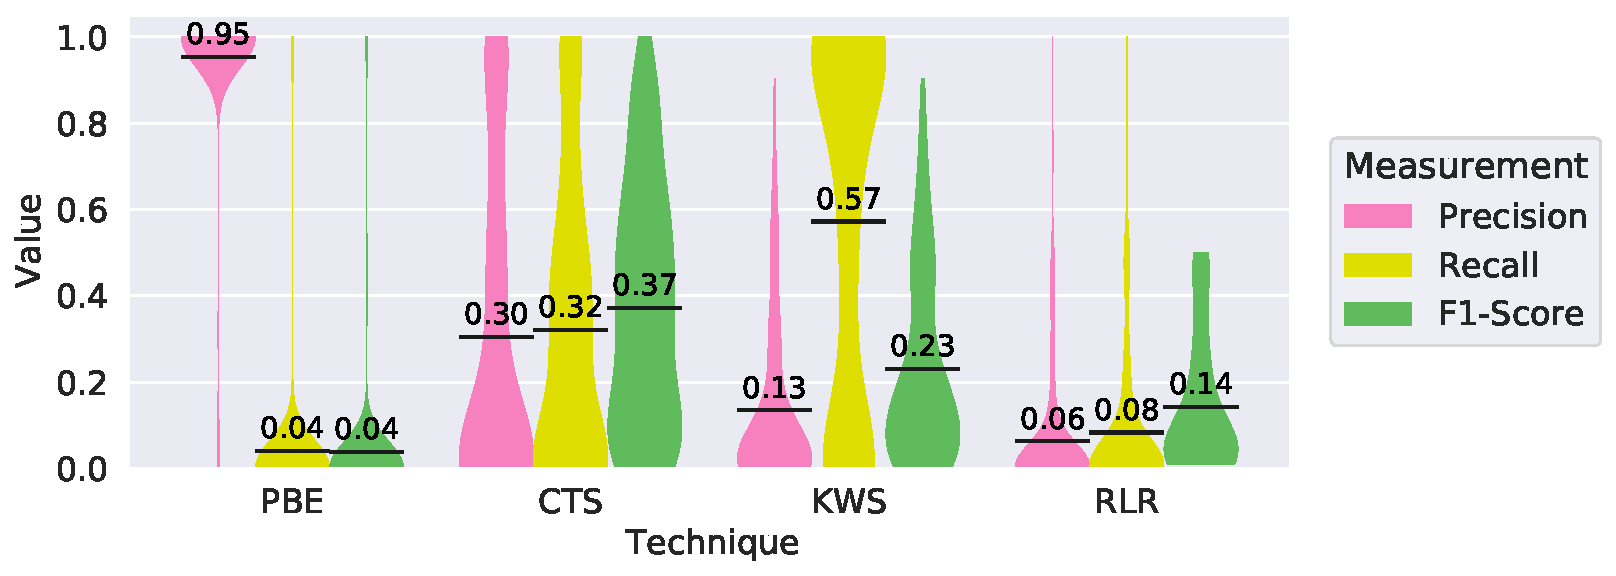
\includegraphics[width=0.75\textwidth, clip]{img/big-study/recall-precision-multicategory-all.pdf}
		\caption{Precision and recall of all techniques compared when training examples are in \emph{more than one} structural categories}
		\label{fig:recall-precision-multicategory-all}
\end{figure}

\subsection{Comparison of All Techniques}
Figure~\ref{fig:success-partial-all} compares the success of all chunk retrieval of the different techniques in our study.
CTS and KWS extract some of the desired lines in 79\% and 88.5\%.
With 38.25\%, KWS also has the highest number of successful extractions, followed by PBE with 34.5\%.
PBE has the lowest number of partial extraction with only 18 out of 400 chunk retrieval runs.

The averaged precision and recall of all techniques is compared in Figure~\ref{fig:recall-precision-all}.
The recall of PBE has a high skew towards one and zero, meaning in most cases either the retrieval is successful or no relevant lines are extracted at all.
Chunk retrieval with CTS has the highest average precision with 46\% and the second best recall with 45\%.
KWS has the smallest precision of the three chunk retrieval techniques.
With 16\% it is still higher than the precision of the RLR baseline with 7\%.
KWS has the highest recall of all techniques with 70\%.

Figure~\ref{fig:recall-precision-singlecategory-all} and Figure~\ref{fig:recall-precision-multicategory-all} show the influence of a single structural category present in the training examples compared to multiple categories present.
For more than one present category, the recall of PBE decreases greatly.
For CTS and KWS the values also decrease, while RLR is not affected by the number of structural categories present.

\end{document}
